\section{Ensretter}\label{sec:ensretter}
Da modtagerspolerne får overført signalet der genereres af frekvensgeneratoren, så vil inputtet til instrumenteringsforstærkeren få en tilnærmet sinus. 
For at undgå det, anvendes en ensretter kreds, for at få et konstant signal.
\begin{figure}[h!]
	\centering
	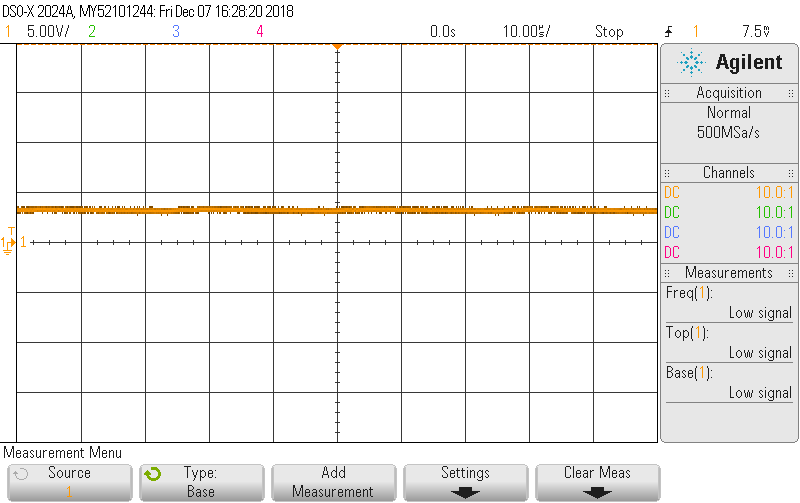
\includegraphics[width=1\textwidth]{billeder/ensretter_png.png}
	\caption{Her ses signalet, efter det er blevet ensrettet.}
	\label{fig:filter_out}
\end{figure}

\subsection{Design}
Enretteren består af en diode, forspændt i lederetningen, der er koblet serielt med en parallelkobling af en spole og en modstand. 
Diodens funktion er at lade halvdelen af signalet passere, hvilket betyder at signalets negative del frafalder. 
For ikke at få et variende positivt pulssignal, indsættes kondensatoren for at glatte spændingen ud. Modstandens funktion er at aflade kondensatoren, så


\husk{Kenneth}{Billede af ensretter kredsløb} 

\subsection{Beregninger}
Til udregning af komponentværdier til ensretteren, antages at en peak spænding på $V_{peak} = 2\si{\volt}$ og der vælges en rippelspænding på 15\% af peakspændingen $V_{rip} = 300 \si{\milli\volt}$
Da der ikke er ligninger nok til at bestemme alle variable, bestemmes afladningsmodstaden til $R_{11} = 5 \si{\kilo\ohm}$
Modstanden og kondensatoren sidder parallelt, hvilket gør at strømmen gennem kondensatoren kan beregnes ved Ohm's lov. Denne strøm bruges både til opladning og afladning.
\begin{align}
	i & = \frac{V_{peak}}{R_{11}} = 400 \si{\mu\ampere}
\end{align}
Den teoretiske værdi for kondensatoren udregnes ved hjælp af ligning 3.36 i bog "\cite[side. 160]{Sedra19uu}".
\begin{align}
	C_{14} & = \frac{V}{V_{rip} \cdot F_c \cdot R_{11}} = 30\si{\nano\farad}
\end{align}
På grund af komponentværdi begræsninger i SMD rækken (E6) på komponentlageret, vælges afladningsmodstanden $R_{11} = 4.7 \si{\kilo\ohm}$, hvoraf en ny teoretisk kondensatorværdi findes $C_{14} = 22 \si{\nano\farad}$.
$\tau$ er tidskonstanten mellem modstanden og kondensatoren, som også er forsinkelsen mellem opladning og afladningen. 
\begin{align}
	\tau & = C_{14} \cdot R_{11} = 22\si{\micro\second}
\end{align}
Da signalet skal ensrettes, skal tidskonstanten, $\tau$ være meget større end periodetiden $T = \frac{1}{F_c}$, for at glatte signalet ud. Periodetiden udregnes til $T = 22 \si{\micro\second}$. Her ses det at $\tau$ og T er lige store. Det er ikke godt, idet kondensatoren når af aflade over en hel periode. Det betyder at $\tau \gg T$, så der tilstræbes et forhold på 20 gange.
Vælges en kondensatorværdi på $C_{14} = 100 \si{\nano\farad}$ fås en ny $\tau = 470\si{\micro\second}$. Forholdet mellem de to størrelser bliver da, 
\begin{align}
	\frac{\tau}{T} & = 21
\end{align}
hvilket svarer til at afladningstiden er 21 gange større end periodetiden. Det er sikrer en lille ripplespænding, hvilket tilnærmelsesvis gør udgangsspændingen til en DC.